\subsection{Theory}

The idea of a decision tree is to split the classifications into a set of decisions.
The first 50 PCA values are used and by looking at the deviance for each split a tree can be created.

\begin{figure}[h]
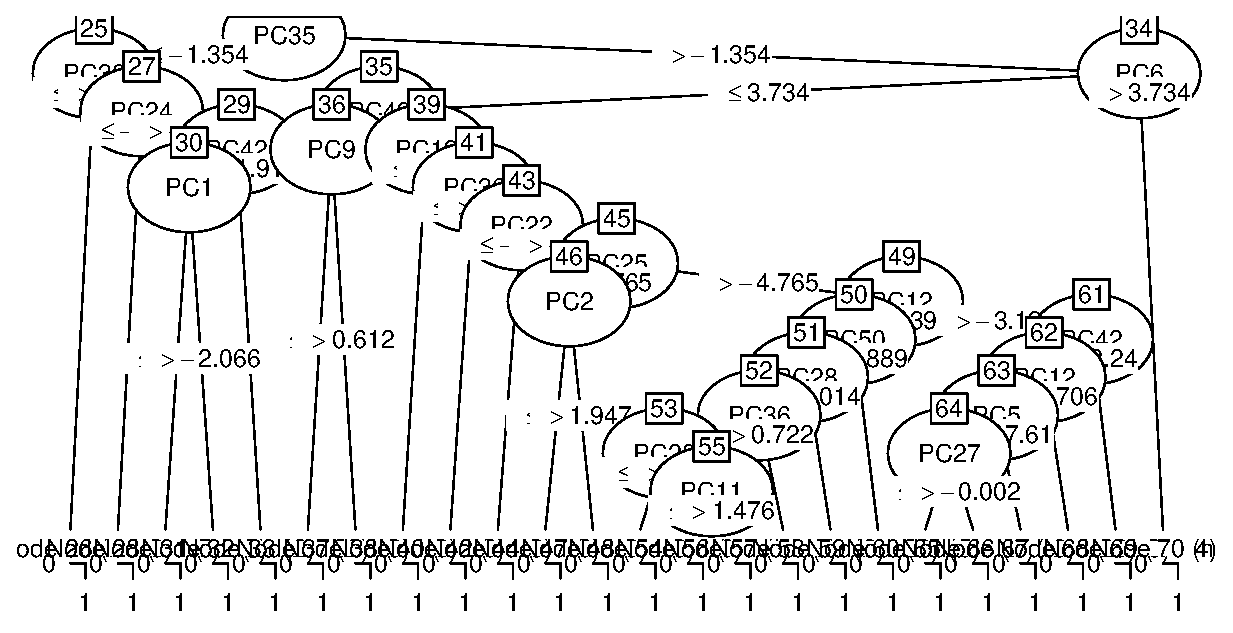
\includegraphics[width = \textwidth]{graphics/tree_section}
\caption[Visualization of a tree.]{Visualization of a small section of the tree.}
\label{fig:tree_section}
\end{figure}

Building a tree can be done using the ``C50'' library in R.
The tree with the training data of 15 people (56000 cases) contains 6338 nodes.
A small section of the tree is shown in figure \ref{fig:tree_section}.
Each node shows which principal component and the split to which the decision is made.
Each leaf shows the probability of a classification.

\begin{figure}[H]
% 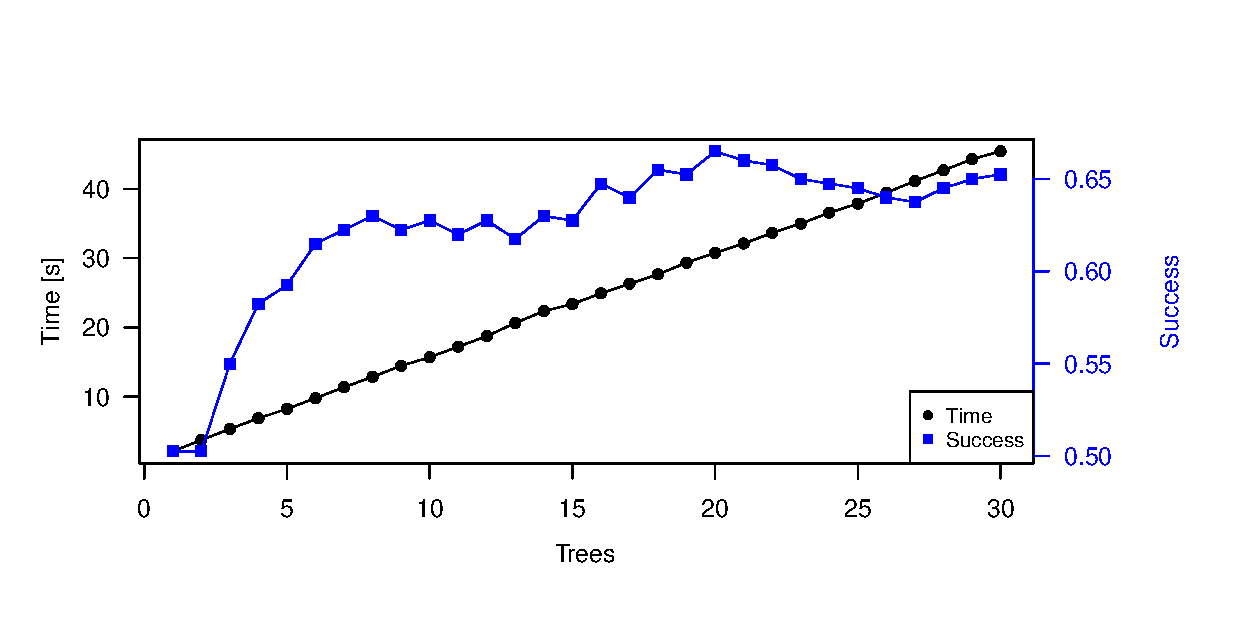
\includegraphics[width = \textwidth]{graphics/tree_timing}
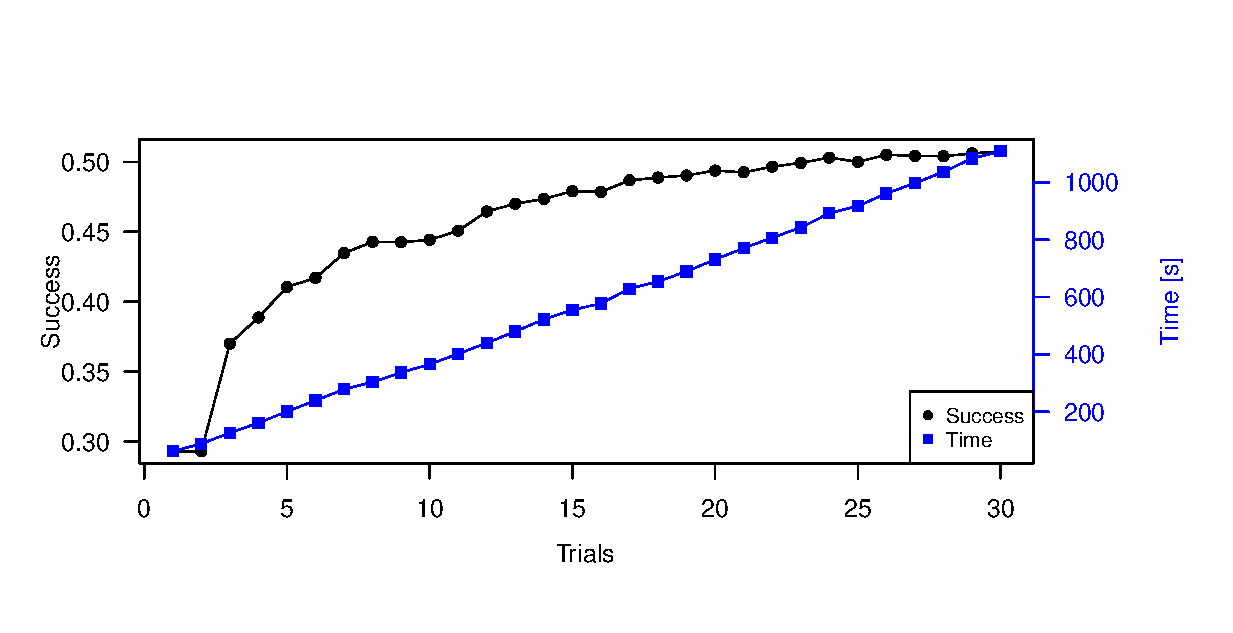
\includegraphics[width = \textwidth]{graphics/tree_timing_entropy}
\missingfigure{also train success to see over fitting}
\caption[Performance of boosting the C50 algorithm.]{Performance of boosting the C50 algorithm. The test person is G3M2 and training data everyone else.}
\label{fig:tree_timing}
\end{figure}

The ``C50'' function provides a boosting function.
Boosting is a process in which the algorithm is training with the train data with multiple trials to increase performance.
This is expected to take more time but improve performance.
In figure \ref{fig:tree_timing} can the success be seen of multiple trials.
Since the algorithm trains towards a good performance on the train data it can't improve beyond a certain point.
The ideal number of boosting trails is set to 15.
The timing is as expected linear dependent on the number of trials.
